\documentclass[aspectratio=169]{beamer}
%[handout]

\usetheme[progressbar=frametitle]{metropolis}
\usepackage{appendixnumberbeamer}

\usepackage[utf8]{inputenc}
\usepackage[T1]{fontenc}

\usepackage[brazil]{babel}
\usepackage[outputdir=..]{minted}
\usepackage{xcolor}
\usepackage{soul} % strikethrough
\usepackage{advdate}
\usepackage{graphicx}
\graphicspath{{figs/}}
\usepackage{graphbox}

\usepackage[ampersand]{easylist}

\usepackage{multirow}
\usepackage{multicol}
\usepackage{subcaption}

\usepackage{pgf,tikz}
\usetikzlibrary{shapes,arrows,positioning}
\usetikzlibrary{circuits.logic.US}
\usetikzlibrary{matrix,calc}

\usepackage{karnaugh-map}

\usepackage{pgfpages}
\setbeameroption{hide notes} % Only slides
% \setbeameroption{show only notes} % Only notes
% \setbeameroption{show notes on second screen=right} % Both

% \graphicspath{{../figs/}}

\definecolor{bgc}{rgb}{0.95,0.9,0.95}
\definecolor{links}{HTML}{2A7F7F}
\hypersetup{colorlinks,linkcolor=,urlcolor=links}

\newminted{verilog}{fontsize=\scriptsize, 
    linenos,
    numbersep=8pt,
    bgcolor=bgc,
    tabsize=4,
    framesep=3mm} 
    %frame=lines,

\newcommand{\verilog}[1]{\verilogf{#1}{\footnotesize}}

\newcommand{\verilogf}[2]{\inputminted[fontsize=#2, 
    linenos,
    tabsize=2,
    numbersep=4pt,
    bgcolor=bgc,
    framesep=3mm]{verilog}{../codes/#1.v}
}

\newminted{nasm}{fontsize=\scriptsize, 
		   linenos,
		   numbersep=8pt,
           bgcolor=bgc,
		   framesep=3mm} 

\usepackage{booktabs}
\usepackage[scale=2]{ccicons}

\usepackage{pgfplots}
\usepgfplotslibrary{dateplot}

\usepackage{hyperref}


\usepackage{xspace}
\newcommand{\themename}{\textbf{\textsc{metropolis}}\xspace}



\usepackage{pifont}% http://ctan.org/pkg/pifont
\newcommand{\cmark}{\ding{51}}%
\newcommand{\xmark}{\ding{55}}%

% \tiny	
% \scriptsize
% \footnotesize
% \small	
% \normalsize	
% \large	
% \Large	
% \LARGE	
% \huge	
% \Huge	



\newminted{python}{fontsize=\scriptsize, 
		   linenos,
		   breaklines,
		   numbersep=8pt,
           tabsize=2,
		   framesep=3mm} 
		   
\newminted{verilog}{fontsize=\scriptsize, 
		   linenos,
		   breaklines,
		   numbersep=8pt,
           tabsize=2,
		   framesep=3mm} 
		   




\definecolor{bgc}{rgb}{0.95,0.9,0.95}
\definecolor{links}{HTML}{2A7F7F}
\hypersetup{colorlinks,linkcolor=,urlcolor=links}


% \usepackage[style=apa]{biblatex}
% \addbibresource{mm.bib}


% \author{\large Prof. Ricardo Menotti (\href{mailto:menotti@ufscar.br}{menotti@ufscar.br})}

\newcommand{\newauthor}[2]{
  \parbox{0.50\textwidth}{
    \texorpdfstring
      {
        \centering
        \small #1 \newline
        {\scriptsize{\urlstyle{same}\href{mailto:#2}{#2}\urlstyle{tt}}}
      }
      {#1} \newline
  }
}

\author{
  \newauthor{Prof. Ricardo Menotti}{menotti@ufscar.br}
\and \newauthor{Prof. Luciano de Oliveira Neris}{lneris@ufscar.br}  
%\and \newauthor{Prof. Artino Quintino da Silva Filho}{artino@ufscar.br}
% \and \newauthor{Prof. Maurício Figueiredo}{mauricio@ufscar.br}
% \and \newauthor{Prof. Edilson Kato}{kato@ufscar.br}
% \and \newauthor{Prof. Roberto Inoue}{rsinoue@ufscar.br}
}

\date{Atualizado em: \today}

\institute{\large \textbf{Departamento de Computação} \\
Centro de Ciências Exatas e de Tecnologia \\
Universidade Federal de São Carlos}

\title{Lógica Digital (1001351)}

\titlegraphic{\hfill
\includegraphics[height=1.5cm]{LogoUfscar}}



\subtitle{Circuitos Sequenciais: Análise de Tempo} % 

\begin{document}

\begin{frame}
	\titlepage
\end{frame} 

\begin{frame}{Temporização de um flip-flop} \centering
    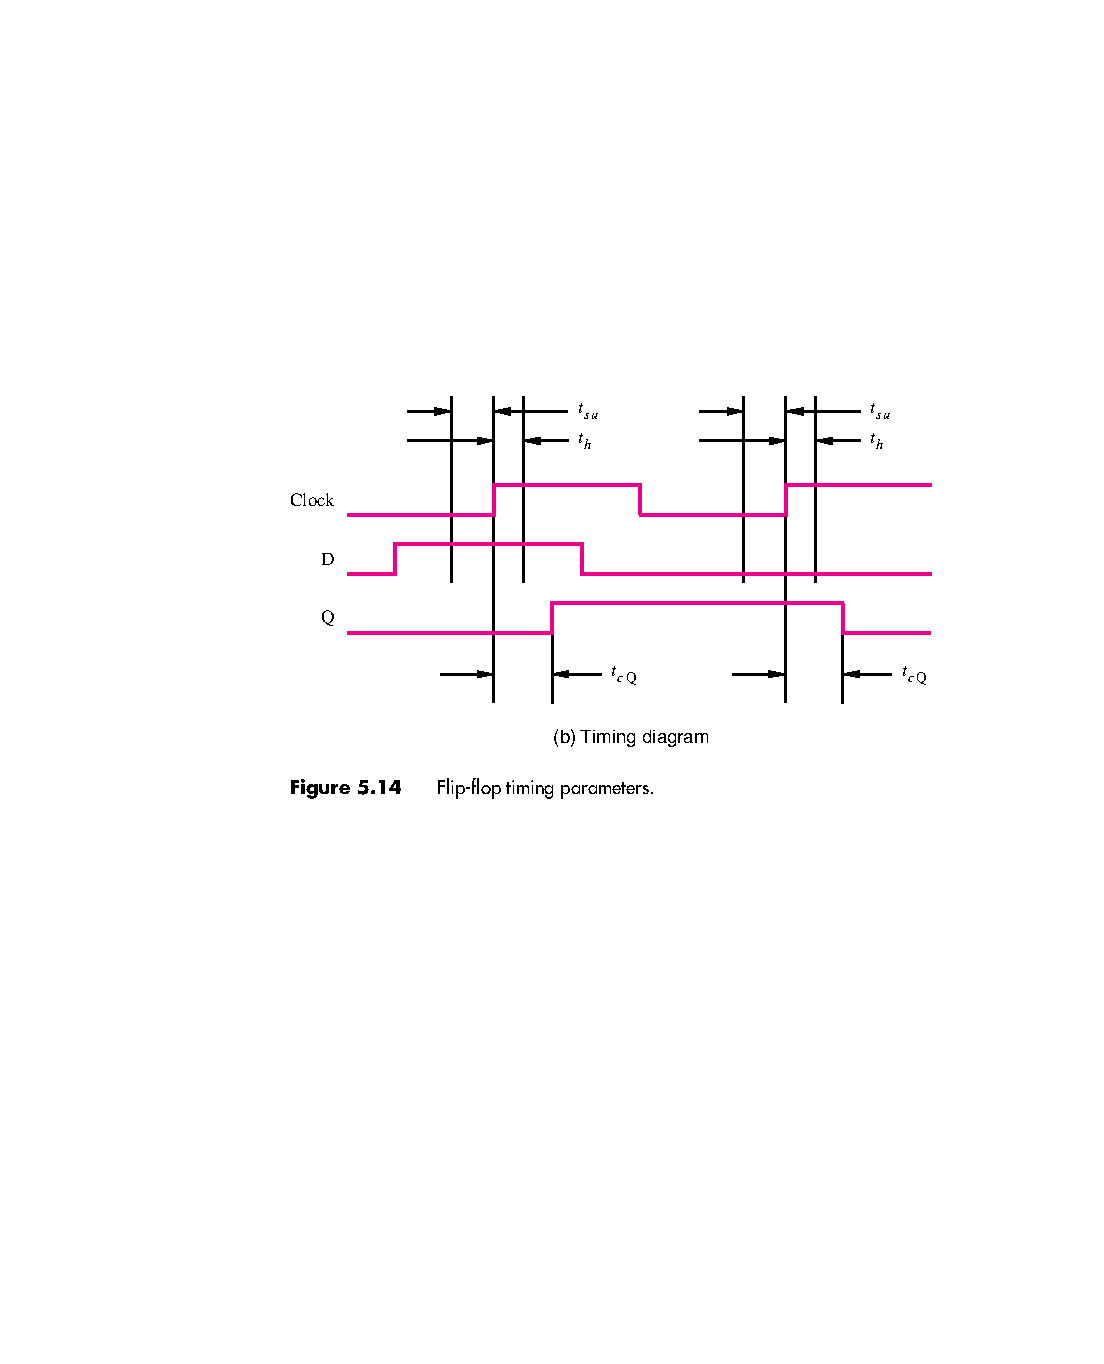
\includegraphics[height=.95\textheight]{VerilogFig5_14} 
\end{frame}

\begin{frame}{Análise de tempo \textit{(timing analysis)}}   \centering
	\begin{columns}
        \column{0.4\textwidth}
            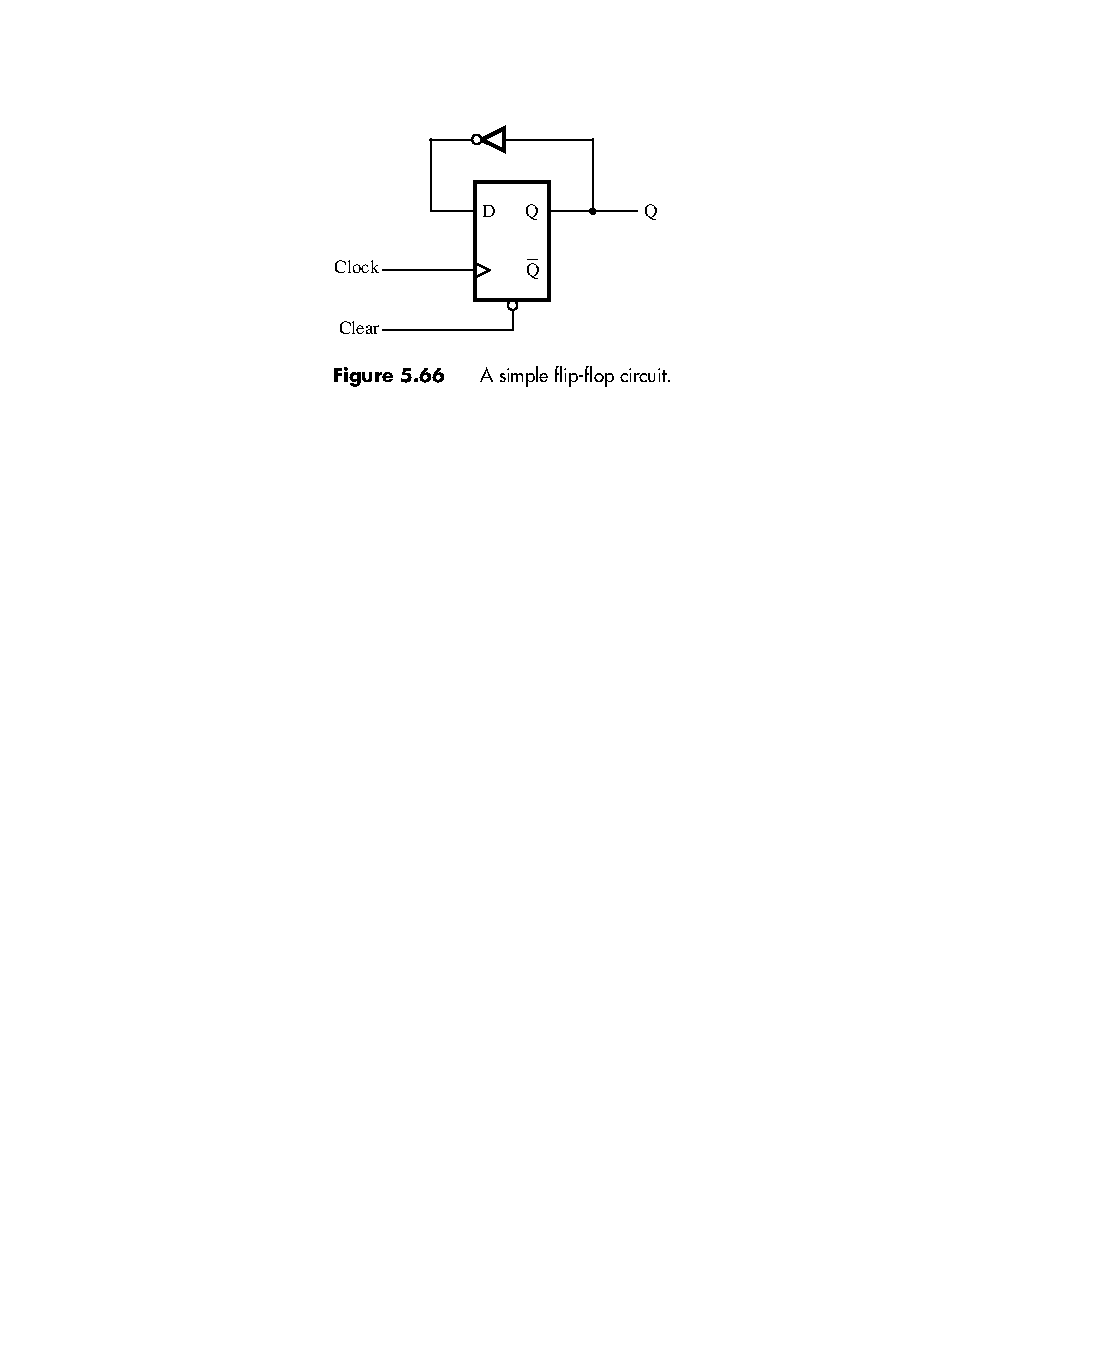
\includegraphics[width=\textwidth]{VerilogFig5_66} 
        \column{0.6\textwidth}
            \begin{itemize}
                \item $t_{su} =$ 0,6 ns
                \item $t_h =$ 0,4 ns
                \item 0,8 ns $\leq t_{cQ} \leq$ 1,0 ns
                \pause
                \item $T_{min} = 1/F_{max}$ 
                \item $T_{min} = t_{cQ} + t_{NOT} + t_{su}$ 
                \item $T_{min} = $ 1,0 $+$ 1,1 $+$ 0,6 $=$ 2,7 ns 
                \item $F_{max} = $ 1$/$2,7 ns $=$ 370,37 MHz
                \pause
                \item $t_{cQ} + t_{NOT} = $ 0,8 $+$ 1,1 $=$ \\ 1,9 ns $> t_h =$ 0,4 ns
            \end{itemize}
    \end{columns}
\end{frame}

\begin{frame}{Análise de tempo \textit{(timing analysis)}}   \centering
	\begin{columns}
        \column{0.45\textwidth}
            \vspace{0.25cm}
            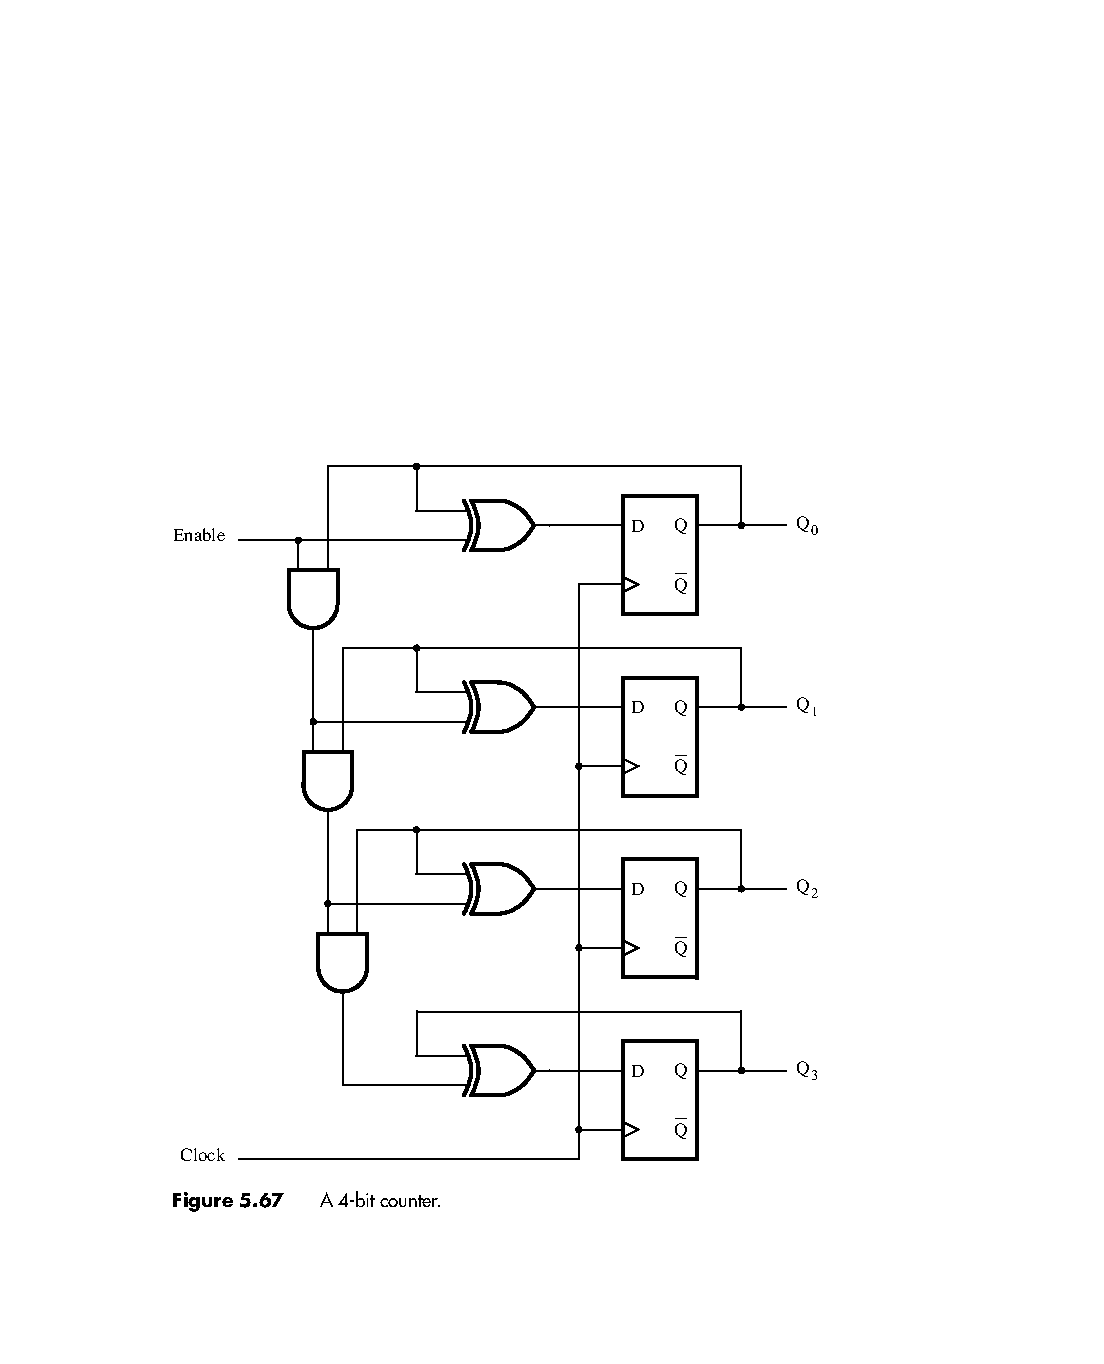
\includegraphics[height=.95\textheight]{VerilogFig5_67} 
        \column{0.55\textwidth}
            \begin{itemize}
                \item $t_{su} =$ 0,6 ns
                \item $t_h =$ 0,4 ns
                \item 0,8 ns $\leq t_{cQ} \leq$ 1,0 ns
                \pause
                \item $T_{min} = 1/F_{max}$ 
                \item $T_{min} = t_{cQ} + 3(t_{AND}) + t_{XOR} + t_{su}$ 
                \item $T_{min} = $ 1,0 $+$ 3(1,2) $+$ 1,2 $+$ 0,6 $=$ 6,4 ns 
                \item $F_{max} = $ 1$/$6,4 ns $=$ 156,25 MHz
                \pause
                \item $t_{cQ} + t_{XOR} = $ 0,8 $+$ 1,2 $=$ \\ 2,0 ns $> t_h =$ 0,4 ns
            \end{itemize}
    \end{columns}
\end{frame}

\begin{frame}{Conceito geral de \textit{clock skew}} \centering
    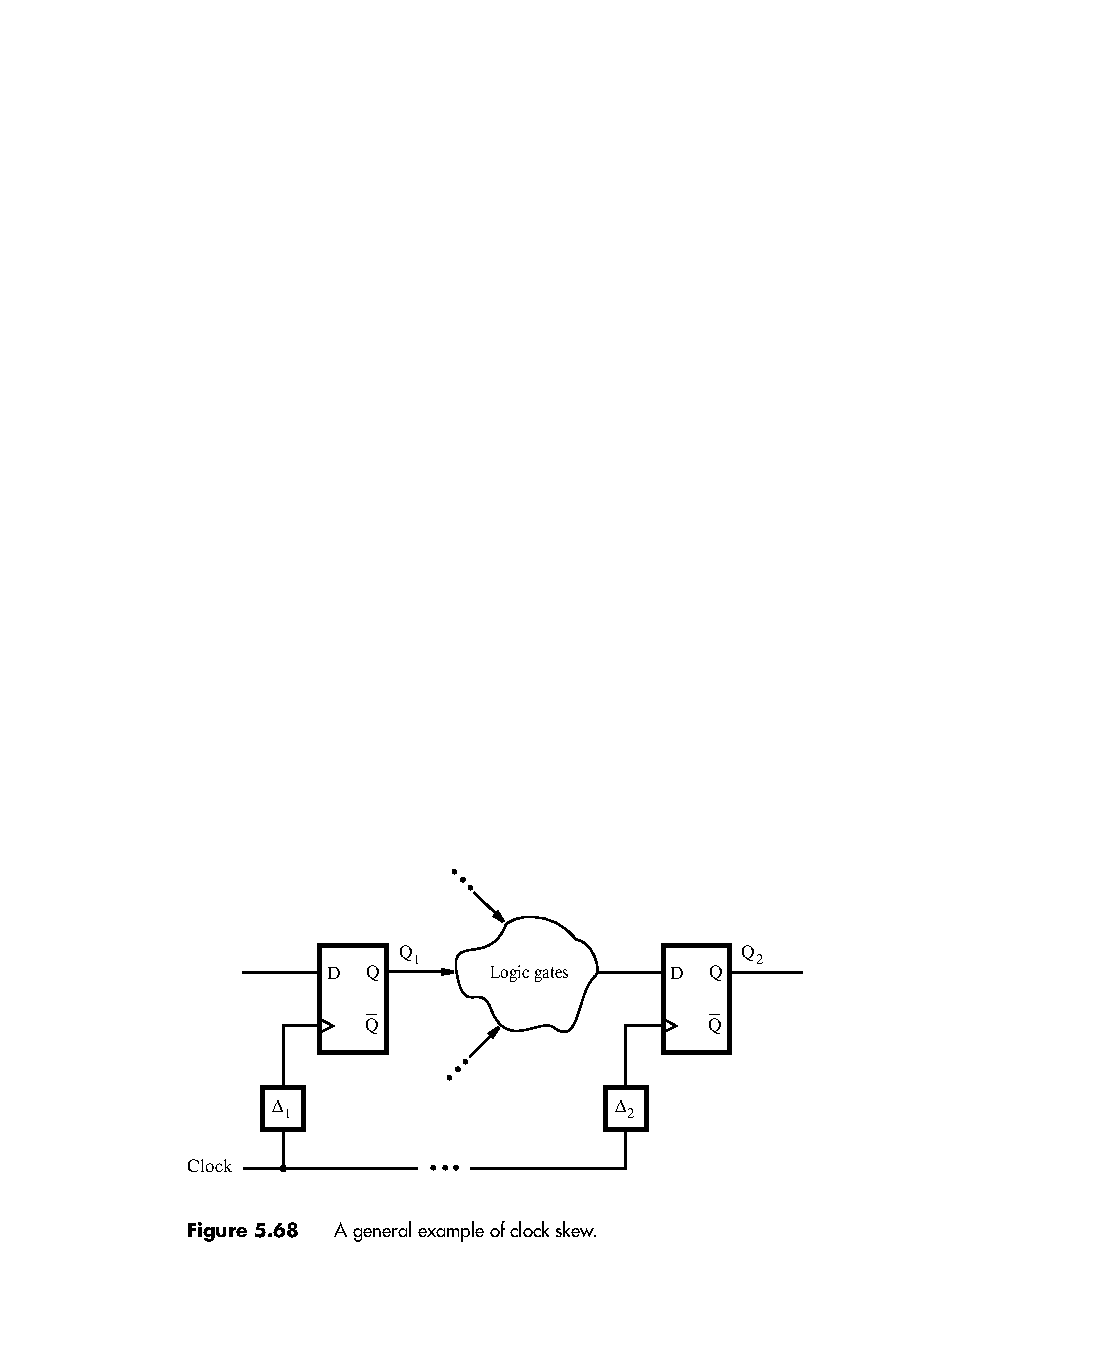
\includegraphics[height=.95\textheight]{VerilogFig5_68} 
\end{frame}

\begin{frame}{Relógio ``distorcido'' \textit{(clock skew)}}   \centering
	\begin{columns}
        \column{0.38\textwidth}
            \vspace{0.5cm}
            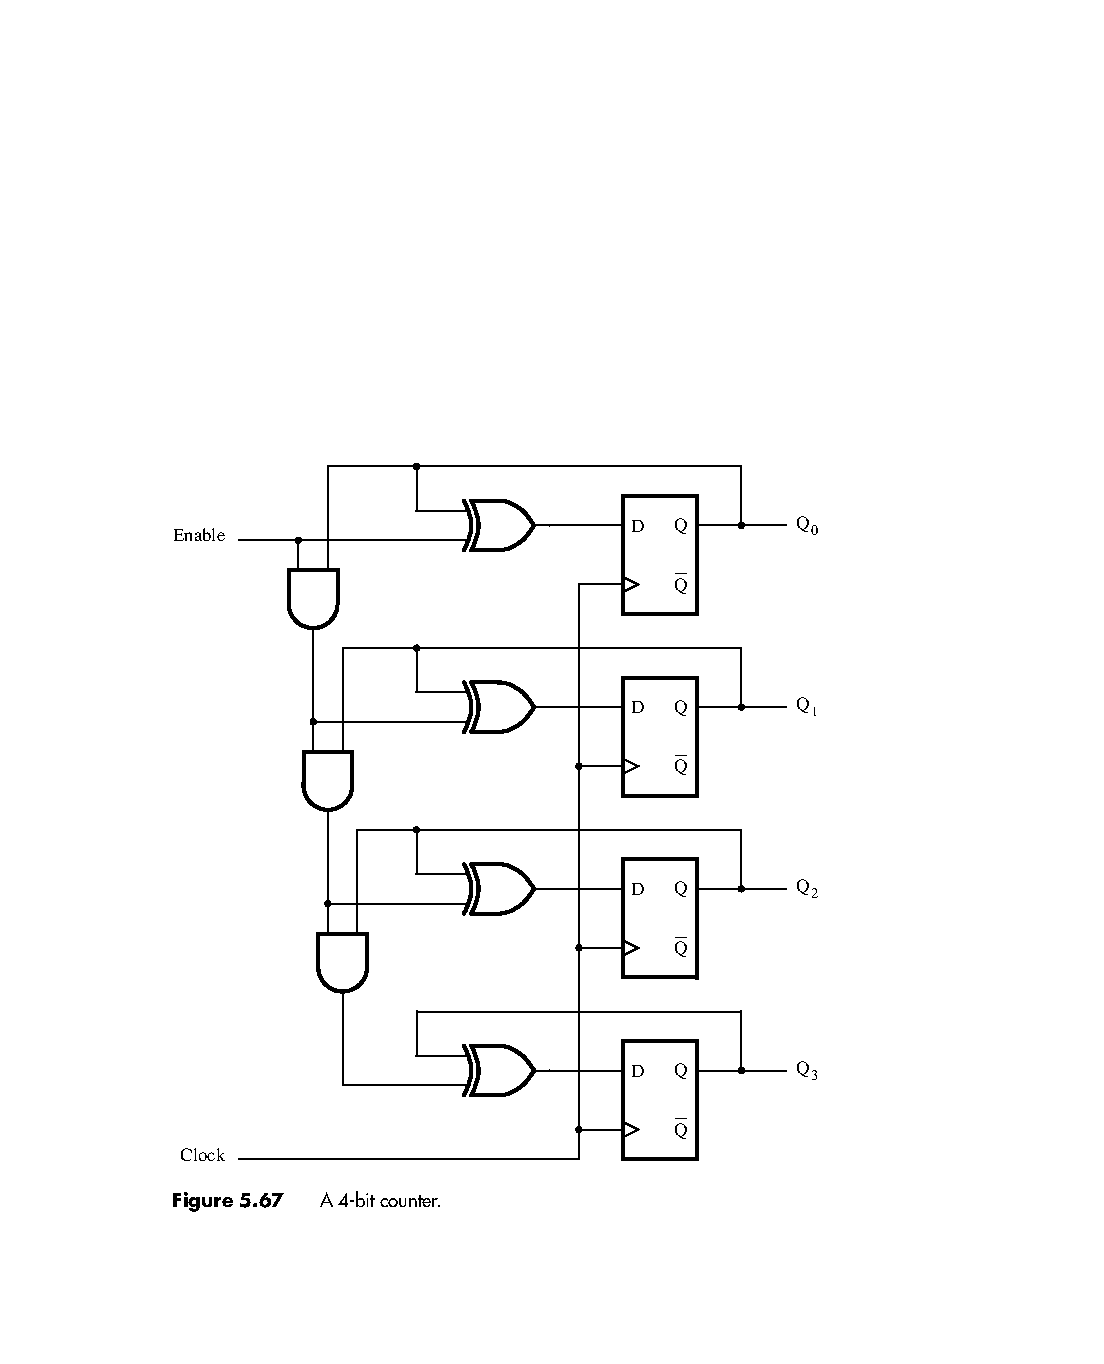
\includegraphics[height=.85\textheight]{VerilogFig5_67} 
        \column{0.63\textwidth}
            \begin{itemize}
                \item $t_{skew} =$ 1,5 ns
                \item $T_{min} = t_{cQ} + 3(t_{AND}) + t_{XOR} + t_{su} - t_{skew}$ 
                \item $T_{min} = $ 1,0 $+$ 3(1,2) $+$ 1,2 $+$ 0,6 $-$ 1,5 $=$ 4,9 ns 
                \item $T_{min} = t_{cQ} + 2(t_{AND}) + t_{XOR} + t_{su}$ 
                \item $T_{min} = $ 1,0 $+$ 2(1,2) $+$ 1,2 $+$ 0,6 $=$ 5,2 ns 
                \item $F_{max} = $ 1$/$5,2 ns $=$ 192,31 MHz
                \pause
                \item $t_{cQ} + t_{AND} + t_{XOR} = $ 0,8 $+$ 1,2 $+$ 1,2 $=$ 3,2 ns $> t_h + t_{skew} = $ 0,4 $+$ 1,5 $=$ 1,9 ns
                \item $t_{skew} \geq $ 2,8 ns
            \end{itemize}
    \end{columns}
\end{frame}

\begin{frame}{Exemplo de análise de tempo} \centering
    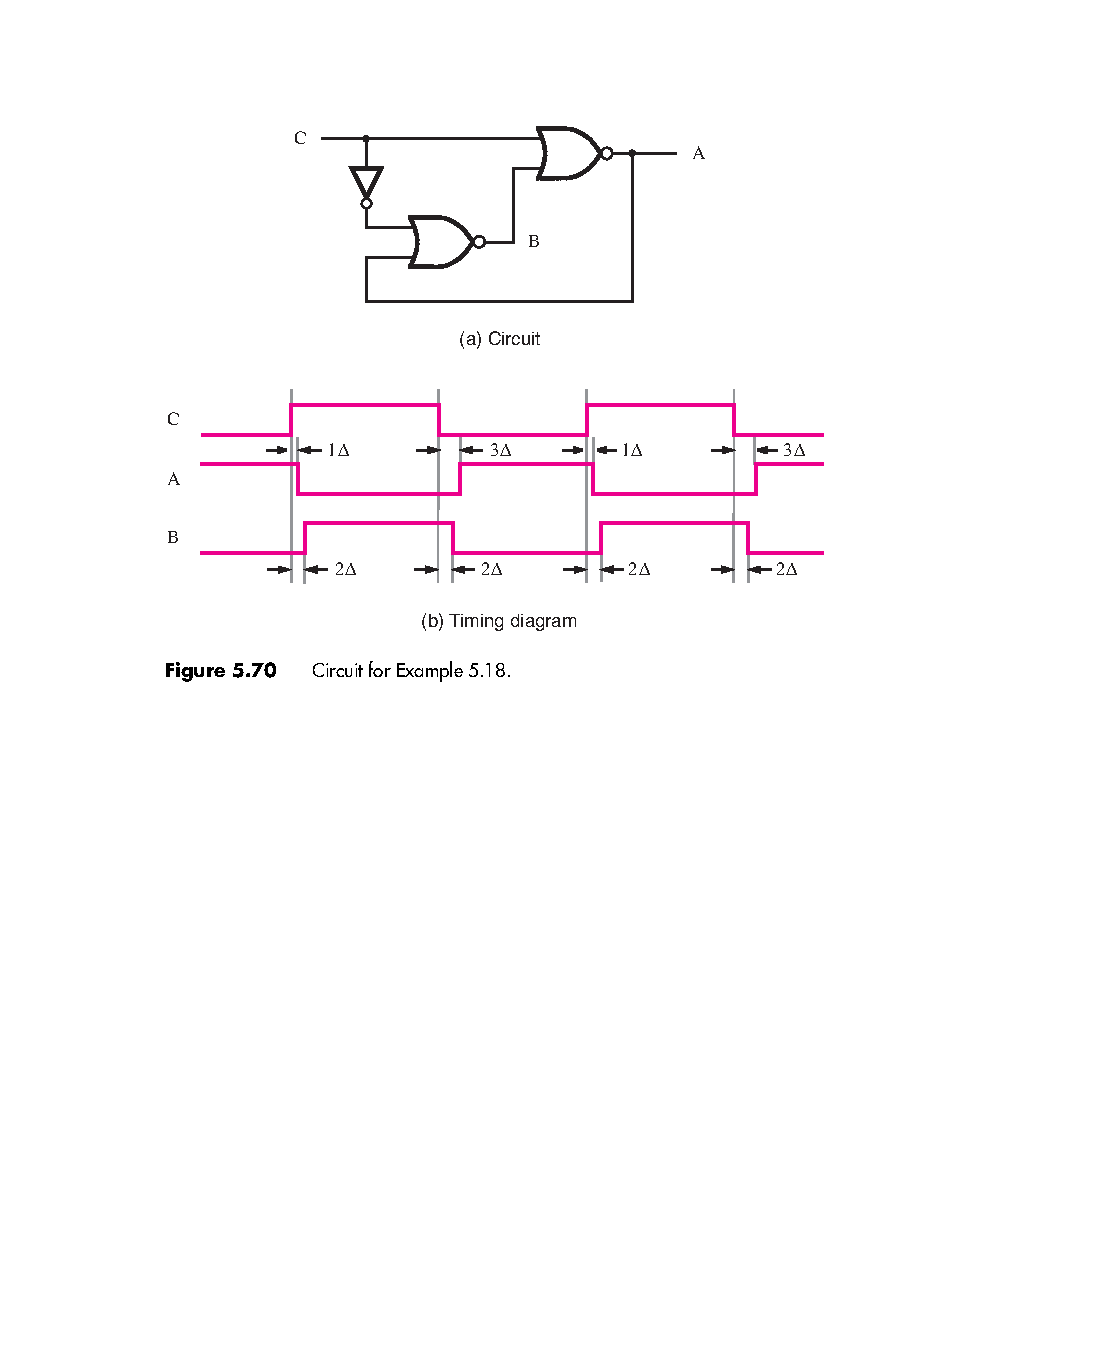
\includegraphics[height=.95\textheight]{VerilogFig5_70} 
\end{frame}

\begin{frame}{Bibliografia} 
	\begin{itemize}
		\item \href{https://www.google.com.br/search?q=filetype\%3Apdf+Fundamentals+of+Digital+Logic+with+Verilog+Design+&oq=filetype\%3Apdf}{Brown, S. \& Vranesic, Z. - Fundamentals of Digital Logic with Verilog Design, 3rd Ed., Mc Graw Hill, 2009}
	\end{itemize}
\end{frame}

\begin{frame}
	\titlepage
\end{frame} 

\end{document}